\newpage
\section{Aufbau}
Zentrale Elemente für den Versuch bilden die zwei Stabpendel welche auf eine Halterung an der Wand in eine Nut aufgelegt sind.
Diese Art der Spitzenlagerung gewährleistet einen möglichst geringen Energieverlust durch Reibung im Vergleich zu anderen Konfigurationen. 
Die Pendel selbst sind zweiteilig und bestehen aus einem Stab mit verschiebbaren Gewicht der jeweiliger Masse von 
\begin{align*}
    M_1 &= \SI{1076,0(1)}{\g}, \\
    M_2 &= \SI{1075,5(1)}{\g}.
\end{align*}
So lässt sich jede gewünschte Pendellänge realisieren durch enstprechendes Verschieben der Gewichte. Im folgenden Versuch wird 
für jede Messung der gleiche Abstand der Massen zur Auflegung eingestellt.
Als Zusatz zu der eigenen Gewichtskraft wird ein Feder, als erweiterte Rückstellkraft, zwischen die Pendel gehängt. 
Diese befindet sich genau dann in Ruhelage, wenn die zwei Pendel nicht ausgelenkt sind. 

\section{Durchführung}
Die Grundkonfiguartion aller drei Messreihen bilden die zwei, auf gleicher Höhe angebrachten Massen. Die Pendellänge sollen also zu jeden Zeitpunkt
gleich sein, wird jedoch in einem zweiten Durchgang zum Vergleich verschoben.



\begin{figure}
    \centering
    \begin{subfigure}[b]{0.3\textwidth}
        \centering
        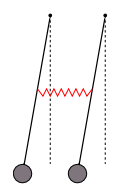
\includegraphics[width=0.6\textwidth]{bilder/gleich.png}
        \caption{Gleichsinnigen Schwingung.}
        \label{fig:4}
    \end{subfigure}
    \hfill
    \begin{subfigure}[b]{0.3\textwidth}
        \centering
         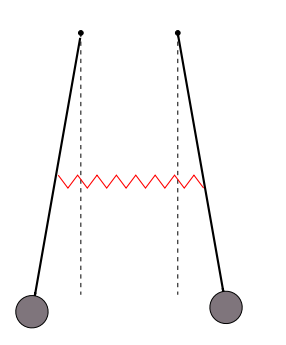
\includegraphics[width=0.6\textwidth]{bilder/gegen.png}
        \caption{Gegenläufigen Schwingung.}
        \label{fig:5}
    \end{subfigure}
    \hfill
    \begin{subfigure}[b]{0.3\textwidth}
        \centering
        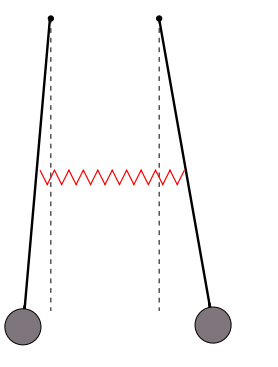
\includegraphics[width=0.6\textwidth]{bilder/koppel.png}
        \caption{Gekoppelte Schwingung.}
        \label{fig:6}
    \end{subfigure}
    \caption{Schematischer Aufbau der verschiedene Konfigurationen. \cite{skript}}
\end{figure}

\subsection{Gleichsinnige Schwingung}
Um die Messwerte der Gleichsinnigen Schwingung zu bestimmen wird zu Beginn die verbindende Feder entnommen und 
die einzelne Schwingdauer $T_i$ der jeweiligen Pendel gewessen. Diese Dauer ist in Abhängigkeit von der Pendellänge, gibt also 
Aufschluss darüber ob die beiden Massen auf der gleichen Höhe angebracht sind, was für die Genauigkeit des Versuches verlangt ist.
Um die Messgenauigkeit besonders bei niedrigen Schwingungsdauern zu erhöhen, werden immmer für jede Messung fünf Schwingungen 
bis zum Stopp der Zeit gewartet. Dieser Vorgang wiederholt sich neun mal um dann mit einem Fehler gemittelt zu werden. 
\\
\newline
Charakteristisch für die Gleichsinnige Schwingung ist die fehlende Dehnung oder Stauchung der Feder, da die Pendel immerzu 
parallel schwingen und an einem Punkt fixiert sind. Deshalb bietet es sich an die Feder zu entfernen um so eventulle Ungenauigkeiten 
vorzubeugen.

%\begin{figure}
%    \centering
%    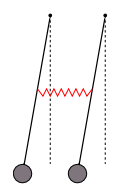
\includegraphics[width=0.3\textwidth]{bilder/gleich.png}
%    \caption{Schematischer Aufbau einer Gleichsinnigen Schwingung. \cite{skript}} 
%    \label{fig:1}
%\end{figure}

\subsection{Gegenläufige Schwingung}
Die zweite Messreihe wird mit der Feder ausgeführt, die an an einer beliebigen Position zwischen den Pendeln aufgehängt wird.
Hier werden die Massen im gleichen Abstand zur jeweiligen Seite ausgelengt und losgelassen. Das System schwingt
folglich Symmetrisch wobei die Feder im Wechsel eine Dehnung und Stauchung erfährt.
Das genaue Ergebnis der Schwingdauer wird nach mehreren Zeitmessungen von jeweils fünf Schwingungen gemittelt.

%\begin{figure}[h!]
%    \centering
%    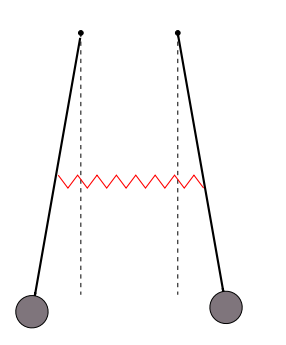
\includegraphics[width=0.3\textwidth]{bilder/gegen.png}
%    \caption{Schematischer Aufbau einer Gegenläufigen Schwingung. \cite{skript}} 
%    \label{fig:2}
%\end{figure}

\subsection{Gekoppelte Schwingung}
Analog zu dem vorherigen Aufbau verbindet die Feder die zwei Pendel miteinander. Um eine asymmetrische Bewegung des Systems 
festellen zu können, wird eine Masse in ihrer Ruhelage gehalten, während die andere ausgelenkt wird.
Die Resultierende Schwingung liefert die Möglichkeit zwei verschiedene Daten aus einem Versuch aufzunehmen.
Zum einem wird die Schwingdauer eines einzelnem Pendel $T$, zum anderen die Schwebungsdauer $T_S$ in einer 
mehrfach ausgeführten Messung über fünf Schwingungen festgestellt.

%\begin{figure}[h!]
%    \centering
%    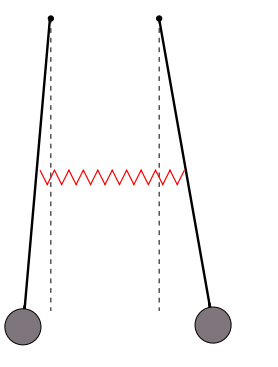
\includegraphics[width=0.3\textwidth]{bilder/koppel.png}
%    \caption{Schematischer Aufbau einer Gekoppelten Schwingung. \cite{skript}} 
%    \label{fig:3}
%\end{figure}



